\chapter{P-value}
To quantify the level of disagreement we compute the P-value
\begin{align}
	P_\mu =\int_{t_\mu}^{\infty}f(t_\mu |\mu) dt_\mu
\end{align}
where $t_\mu$  is the value of the statistic $t_\mu$ observed from the data and $f(t\mu |\mu)$ denotes
the PDF (Probability density function) of t$_\mu$ under the assumption of the signal strength $\mu$
\begin{align}
	f(t\mu |\mu)=\frac{1}{\sqrt{2\pi}} \frac{1}{\sqrt{t_\mu}}e^\frac{-t_\mu}{2}
\end{align}


\begin{figure}
	\centering
	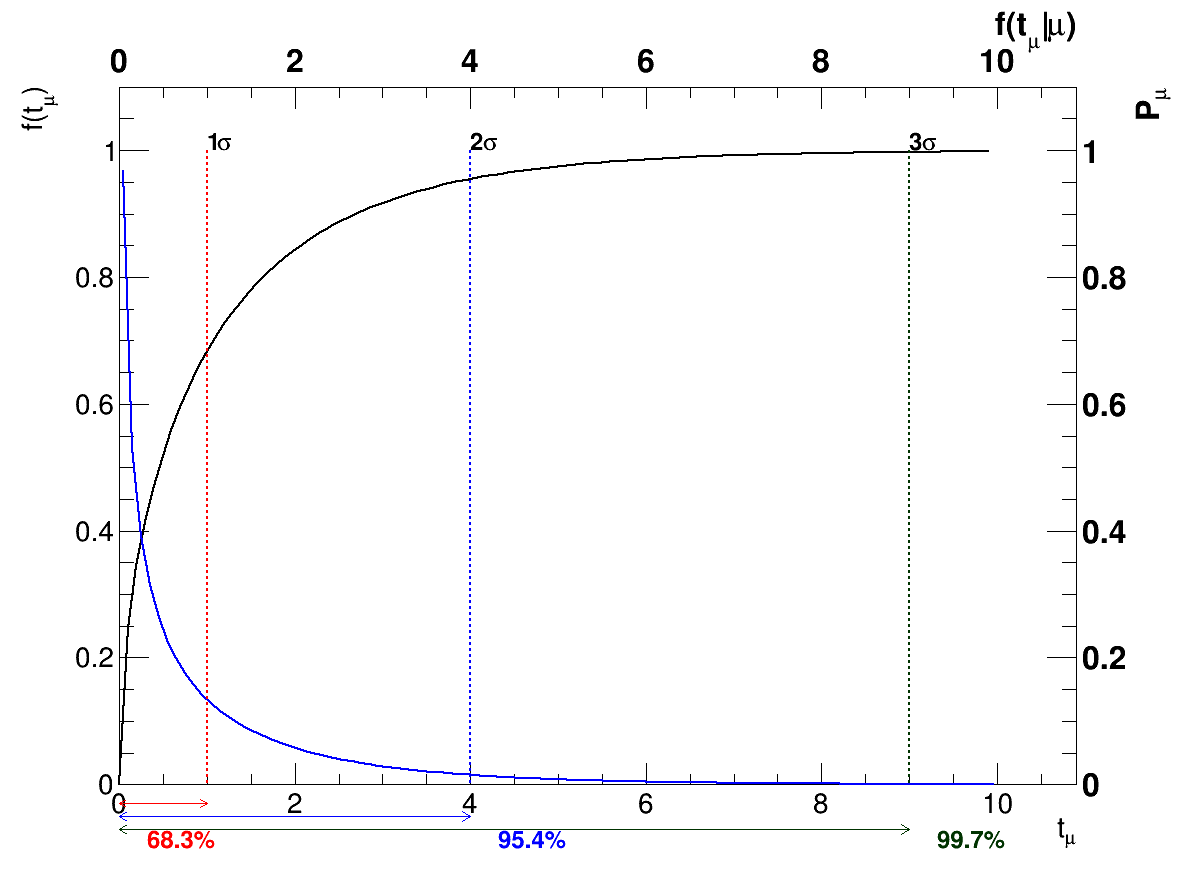
\includegraphics[width=9cm,height=6	cm]{Chapter3/nos.png}
	\caption{Prueba estad\'istica de $t_\mu$ y P valor para $t_\mu$}
\end{figure}
%valores de sigma en 1,4, 9 corresponden a las areas de una gaussiana en isigma,2sigma y 3 sigma


\begin{figure}
	\centering
	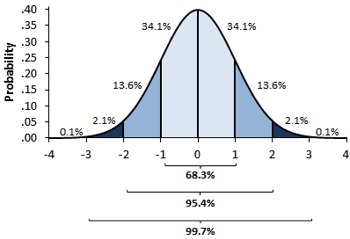
\includegraphics[width=9cm,height=6cm]{Chapter3/normal-curve.jpg}
	\caption{Distribuci\'on gaussiana que ilustra los valores de significancia y su probabilidad}
\end{figure}